\section{Time Step Length in the N-body Problem}
\label{sec:TimeStepLengthNbody}
When estimating the time step length required to study the evolution of the star cluster consisting of $N=100$ particles initially uniformly distributed in a sphere of radius $20$ ly with normal distributed masses with mean $10{\textrm{M}}_{\odot}$, the initial and final distribution of particles in the radial direction for a finite time period is studied for different time step lengths. 
The time period, considered, is chosen to be of the order of the characteristic time $\tau _{crunch}$, given in \matref{eq:t_crunch}.
$\tau _{crunch}$ is the finite time at which the system with $N \rightarrow \infty$ particles with no or low initial velocity collapses into a singularity. \fxnote{ref!}
\begin{align}
	\tau _{crunch} = \sqrt{\frac{3\pi}{32G\rho_0}}
	\label{eq:t_crunch}
\end{align}
With the units light years, years and solar masses ${\textrm{M}}_{\odot}$, the value of the gravitational constant is, according to \secref{sec:Conversion}, $G = 1.536\cdot 10^{-13} \textrm{ly}^3 / \textrm{yr}^2 {\textrm{M}}_{\odot}$, whilst the mass density of $N=100$ particles with a mean mass of $10 {\textrm{M}}_{\odot}$ within the sphere of radius $20 \text{ly}$ is 
$\rho_0 = 10 {\textrm{M}}_{\odot} / (4/3 \pi (20 \text{ly})^2)$, yielding that the $\tau _{crunch}$ becomes
\begin{align}
	\tau _{crunch} = \sqrt{\frac{12\pi^2\cdot 20^3}{32\cdot 1.536\cdot 10^{-13}}\cdot 10\cdot 3} \text{ yr} 
	\approx 8.0\times 10^7 \text{ yr}
\end{align}
The histograms in \figref{fig:histograms_VV_diff_time_step} and \ref{fig:histograms_RK4_diff_time_step} show the initial and final radial position of 100 particles in a sphere of radius $20$ ly, initially at rest, interacting only through the Newtonian force between all particles, after $10^7$ years with different step lengths. 
The masses and initial position of the 100 particles are generated by the functions given in \secref{Method:GeneratingPosMassVel}.
the final positions given in the histograms of \figref{fig:histograms_VV_diff_time_step} are computed with the Velocity-Verlet method for N bodies, whilst the final positions given in the histograms of \figref{fig:histograms_RK4_diff_time_step} are computed with the fourth order Runge-Kutta method for N bodies.
\begin{figure}[H]
\centering
\begin{minipage}{.5\textwidth}
  \centering
  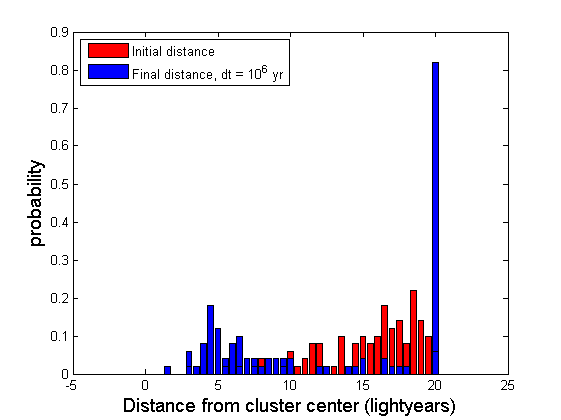
\includegraphics[width=1\linewidth]{Figures/graphs_VV/pos1_VV.png}
\end{minipage}%
\begin{minipage}{.5\textwidth}
  \centering
  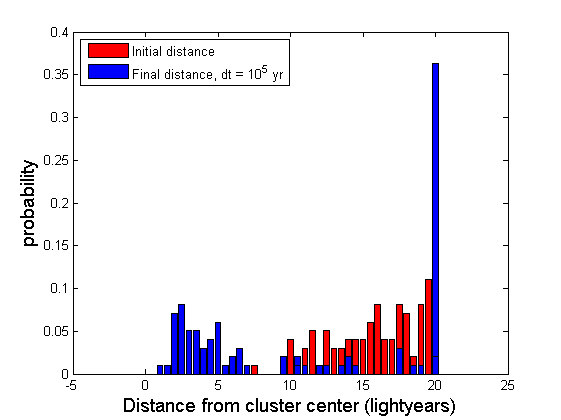
\includegraphics[width=1\linewidth]{Figures/graphs_VV/pos2_VV.png}
\end{minipage}
\begin{minipage}{.5\textwidth}
  \centering
  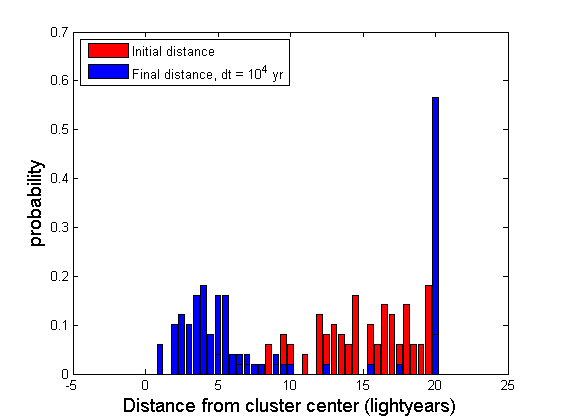
\includegraphics[width=1\linewidth]{Figures/graphs_VV/pos3_VV.png}
\end{minipage}%
\begin{minipage}{.5\textwidth}
  \centering
  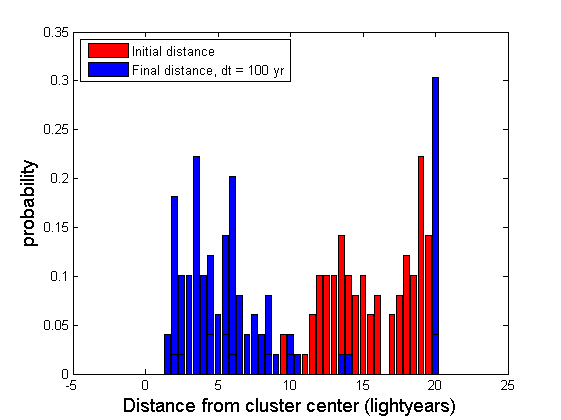
\includegraphics[width=1\linewidth]{Figures/graphs_VV/pos5_VV.png}
\end{minipage}
\caption{
Initial and final position position over a time period of $10^7$ years for 100 particles in a sphere of radius $20$ ly computed by the Velocity-Verlet method, for different time step lengths $dt$.
The masses of the particles are normal distributed around $10{\textrm{M}}_{\odot}$ with a standard deviation of $1{\textrm{M}}_{\odot}$, whilst the initial positions are computed from an initial uniform density within the sphere.
The depicted particle probability at the distance $r=20$ ly correspond to particles that are actually at around $20$ ly away from the cluster center after $10^7$ years, but it also accounts for the particles that has escaped the cluster, that is $R>20$ ly.
}
\label{fig:histograms_VV_diff_time_step}
\end{figure}
By comparing the four histograms in \figref{fig:histograms_VV_diff_time_step} for different time step lengths, in seems that the final radial distribution of the particles after $10^7$ years consists of three distinct features. Close to the center, at a distance smaller that $5-10$ ly, a high density seems to appear. 
In addition a great part of the particles seem to be ejected from the cluster. 
This is seen by the high probability bar at a distance $R=20$ ly from the cluster center. This bar represents both particles at the edge of the cluster and particles that have been ejected from the cluster. 
For long time steps, this ejection seems to be greater than for short time steps.
That is, for a step length of $dt = 10^6$ yr, the amount of particles that has been ejected from the cluster after $10^7$ yr is roughly $40 \%$, whilst the amount of ejected particles with a step length of $dt = 100$ years is only around $15 \%$.
This is similar to the result gained in \secref{sec:stability2bodysystem}, where the distance between the bodies after 100 years in the Sun-Earth-like system was computed to be greater for larger time step lengths than for short time step lengths for the Velocity-Verlet method, as well, as seen in \figref{fig:SunEarthDistanceAfter100yr}. 
The third feature of the histograms in \figref{fig:histograms_VV_diff_time_step} is the small density of particles at more than $10$ ly away from the cluster center.
All of the histograms with different time step lengths show these same features, apart from the number of ejected particles, which vary rapidly with decreased step length. 
\begin{figure}[H]
\centering
\begin{minipage}{.5\textwidth}
  \centering
  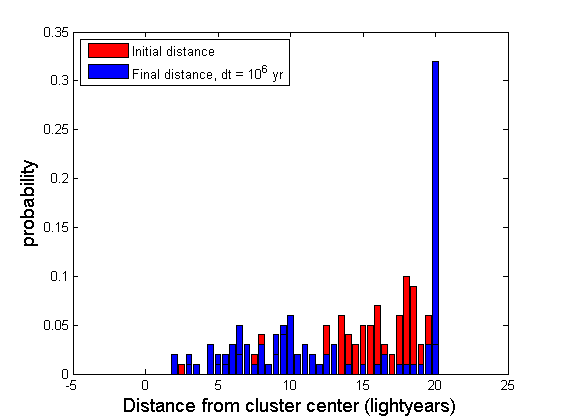
\includegraphics[width=1\linewidth]{Figures/graphs_RK4/pos6.png}
\end{minipage}%
\begin{minipage}{.5\textwidth}
  \centering
  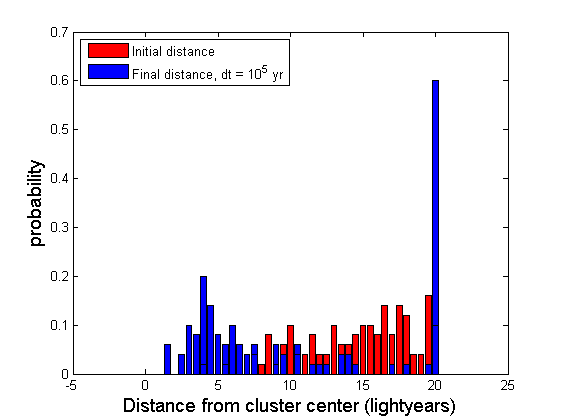
\includegraphics[width=1\linewidth]{Figures/graphs_RK4/pos5.png}
\end{minipage}
\begin{minipage}{.5\textwidth}
  \centering
  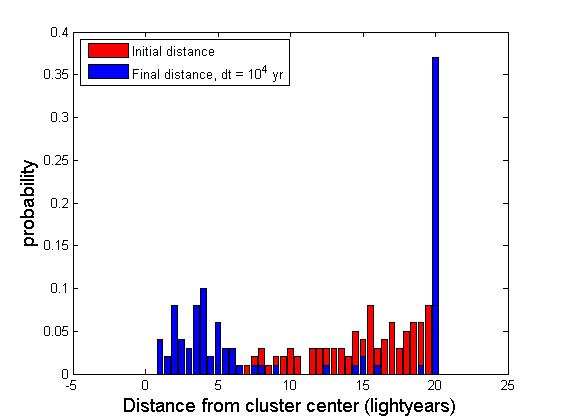
\includegraphics[width=1\linewidth]{Figures/graphs_RK4/pos4.png}
\end{minipage}%
\begin{minipage}{.5\textwidth}
  \centering
  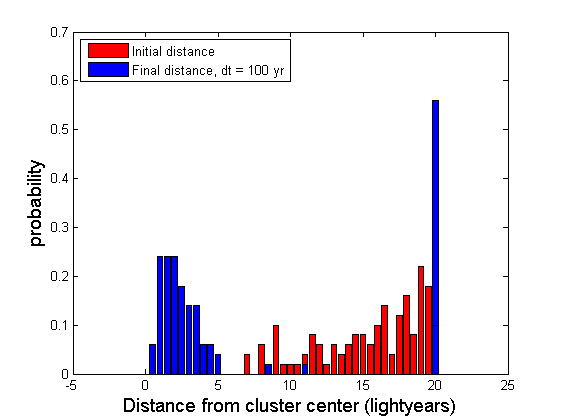
\includegraphics[width=1\linewidth]{Figures/graphs_RK4/pos9.png}
\end{minipage}
\caption{
Initial and final position position over a time period of $10^7$ years for 100 particles in a sphere of radius $20$ ly computed by the Fourth order Runge-Kutta method, for different time step lengths $dt$.
The masses of the particles are normal distributed around $10{\textrm{M}}_{\odot}$ with a standard deviation of $1{\textrm{M}}_{\odot}$, whilst the initial positions are computed from an initial uniform density within the sphere.
The depicted particle probability at the distance $r=20$ ly correspond to particles that are actually at around $20$ ly away from the cluster center after $10^7$ years, but it also accounts for the particles that has escaped the cluster, that is $R>20$ ly.
}
\label{fig:histograms_RK4_diff_time_step}
\end{figure}
\fxnote{is it ok that I have just copy-pasted caption??}

As for the radial distribution after $10^7$ years computed by the Velocity-Verlet method, the final distribution shown in \figref{fig:histograms_RK4_diff_time_step}, computed by the fourth order Runge-Kutta method, show the three features: high density close to the center, low density at a more than $10$ ly from the center, and an ejection of particles from the cluster.
However, for long time steps, that is $dt = 10^6$ yr, these features are not as distinct, yielding that this step length is too long for the Runge-Kutta method. 
Unlike the Velocity-Verlet method, the amount of particles that are ejected from the cluster using the Runge-Kutta method seems, however, to be stable for all depicted step lengths at around $30 \%$. 

In the two particle case the Velocity-Verlet method seemed like it was the most stable method over time. Looking at the N particle case the Velocity-Verlet is more dependent of the choice of time step, whilst the Runge-Kutta 4 method is more stable towards the change in time-step. This might have a lot to say for the stability of the system and the computational time. Therefore the Runge-Kutta 4 method seems like the better choice when looking at times greater than $\tau_{crunch}$. 



After finding the positions of the particles after a time in the order of a $\tau_{crunch}$, the star cluster have not collapsed into a mass in the middle. Therefore using $\tau_{crunch}$ as a unit of time to study the further behaviour is a natural conclusion. For this to work the gravitational constant has to be transformed into units that fits and for the N particle case. Using \matref{eq:t_crunch} it's possible to find the gravitational constant as a function of particles N.  
\begin{align}
G = 986.96 \frac{1}{N} \frac{\textrm{ly}^3}{\tau_{crunch}^2\textrm{m}_{mean}}
\end{align}

Now when looking at timescales larger than $\tau_{crunch}$, the time steps have to be calculated from the new unit of time $\tau_{crunch}$. From the histograms in \figref{fig:histograms_RK4_diff_time_step} the best time step length to choose is $10^5$ years. If this is then transformed into the new time scale it is
\begin{align*}
dt = 10^{-3} \tau_{crunch}
\end{align*}
